% begin module derivatives-as-function-ex2
\begin{frame}
\begin{example}
If $f(\alertNoH{3,4}{x}) = {\alertNoH{3,4}{x}}^3-{\alertNoH{3, 4}{x }}$, find formula for $f'(x)$.
\begin{columns}[c]
\column{.25\textwidth}
\psset{xunit=0.7cm, yunit=0.7cm}
\begin{pspicture}(-2,-2.5)(2,2.5)
\psframe*[linecolor=white](-2,-2.5)(2,2.5)
\psaxes[ticks=none, labels=none]{<->}(0,0)(-2,-2.5)(2,2.5)
%Function formula: - (x)+(x)^{3}
\psplot[linecolor=red, plotpoints=1000]{-1.5}{1.5}{x 3 exp x -1 mul add }
\tiny
\fcLabelXOne
\fcLabelYOne
\rput[l](-1.3, 0.6){$y=f(x)=x^3-x$}
\end{pspicture}
%\ 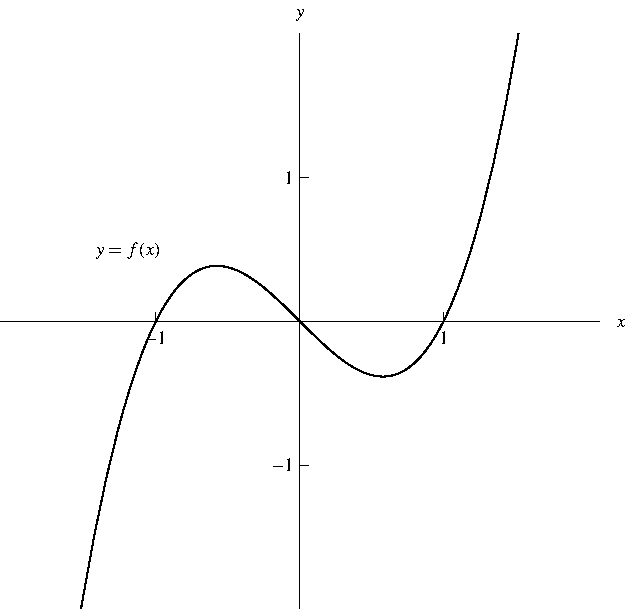
\includegraphics[height=3cm]{derivatives/pictures/03-02-ex2a.pdf}%
%\ \only<handout:0| -7>{%
%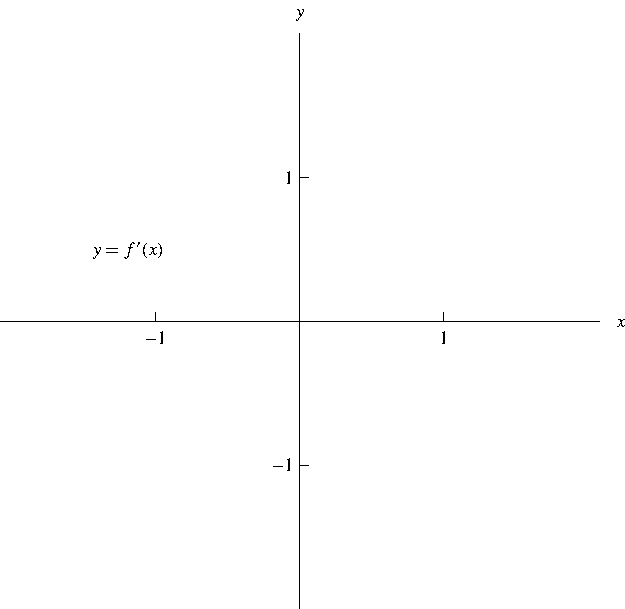
\includegraphics[height=3cm]{derivatives/pictures/03-02-ex2b.pdf}%
%}%
%\only<8->{%
%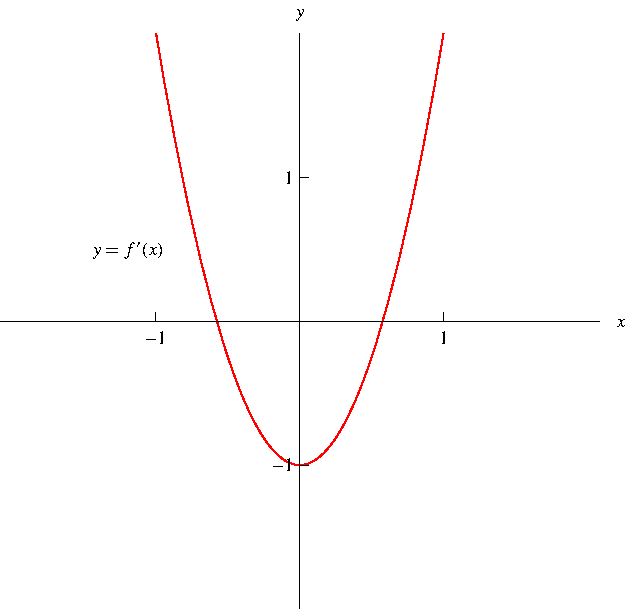
\includegraphics[height=3cm]{derivatives/pictures/03-02-ex2c.pdf}%
%}%

\psset{xunit=0.7cm, yunit=0.7cm}
\begin{pspicture}(-2,-2.5)(2,2.5)
\psframe*[linecolor=white](-2,-2.5)(2,2.5)
\psaxes[ticks=none, labels=none]{<->}(0,0)(-2,-2.5)(2,2.5)
\tiny
\fcLabelXOne
\fcLabelYOne
%Function formula: 3 ((x)^{2})-1
\uncover<13->{
\psplot[linecolor=blue, plotpoints=1000]{-1}{1}{-1 x 2 exp 3 mul add }
\rput[l](-1.3, -1.5){$y=f'(x)=3x^2-1$}
}
\end{pspicture}
\column{.75\textwidth}
$
\begin{array}{@{}r@{}c@{}l}
\uncover<2->{f'(x)} & \uncover<2->{ = } &\displaystyle \uncover<2->{\lim_{h\rightarrow 0} \frac{f( \alertNoH{3}{ x+h} )-f(\alertNoH{4}{x})}{h}}\\%
& \uncover<3->{ = } &\displaystyle \uncover<3->{ \lim_{h \rightarrow 0} \frac{\alertNoH{7,8}{ (\alertNoH{3}{x+h})^3}\alertNoH{5}{ - (\alertNoH{3}{x+ h})} \alertNoH{6}{ -\left({\alertNoH{4}{x}}^3-{\alertNoH{4}{x}} \right)}}{h}}\\%
& \uncover<5->{ = } &\displaystyle \uncover<5->{ \lim_{h \rightarrow 0} \frac{ \fcAnswerUncover{5}{8}{ \fcCancel{9}{x^3} + 3x^2h +3xh^2+h^3} \alertNoH{5}{-\fcCancel{9}{x}-h} \alertNoH{6}{-\fcCancel{9}{x^3}+\fcCancel{9}{x}} }{h}}\\%
& \uncover<9->{ = } &\displaystyle \uncover<9->{ \lim_{h \rightarrow 0} \frac{3x^2\alertNoH{10}{h}+3x{\alertNoH{10}{h}}^2+{\alertNoH{10}{h}}^3-{\alertNoH{10}{h}}}{h}}\\%
& \uncover<10->{ = } &\displaystyle \uncover<9->{ \lim_{h \rightarrow 0} \frac{\fcCancel{11}{\alertNoH{10}{h}}(3x^2+3xh+ h^2-1) }{ \fcCancel{11}{h}}}\\%
& \uncover<11->{ = } &\displaystyle \uncover<11->{ \alertNoH{12,13}{\lim_{h \rightarrow 0} (3x^2+3xh+h^2-1)}}\\%
& \uncover<12->{\alertNoH{12,13} {=} } &\displaystyle \fcAnswer{13}{3x^2-1}%
\end{array}
$
\end{columns}
\end{example}
\end{frame}
% end module derivatives-as-function-ex2
